\documentclass[onecolumn, draftclsnofoot, 10pt, compsoc]{IEEEtran}
\usepackage{graphicx}
\usepackage{url}
\usepackage{setspace}
\usepackage{geometry}

\geometry{textheight=9.5in, textwidth=7in}

% 1. Fill in these details
\def \CapstoneTeamName{			Team Name TBD}
\def \CapstoneTeamNumber{		41}
\def \GroupName{				30k CS Avionics}
\def \GroupMemberOne{			Joshua Novak}
\def \GroupMemberTwo{			Allison Sladek}
\def \GroupMemberThree{			Levi Willmeth}
\def \CapstoneProjectName{		30K Rocket Spaceport America}
\def \CapstoneSponsorCompany{	Oregon State University}
\def \CapstoneSponsorPerson{	Dr. Nancy Squires}

% 2. Uncomment the appropriate line below so that the document type works
\def \DocType{		%Problem Statement
					Requirements Document
					%Technology Review
					%Design Document
					%Progress Report
				}
			
\newcommand{\NameSigPair}[1]{
	\par
	\makebox[2.75in][r]{#1} \hfill
	\makebox[3.25in]{\makebox[2.25in]{\hrulefill} \hfill \makebox[.75in]{\hrulefill}}
	\par\vspace{-12pt}
	\textit{
		\tiny\noindent \makebox[2.75in]{} \hfill
		\makebox[3.25in]{\makebox[2.25in][r]{Signature} \hfill \makebox[.75in][r]{Date}}
	}
}
% 3. If the document is not to be signed, uncomment the RENEWcommand below
%\renewcommand{\NameSigPair}[1]{#1}
% \renewcommand{\thesubsubsection}{\thesection.\alph{subsubsection}}

%%%%%%%%%%%%%%%%%%%%%%%%%%%%%%%%%%%%%%%
\begin{document}
\begin{titlepage}
    \pagenumbering{gobble}
    \begin{singlespace}
    	%\includegraphics[height=4cm]{coe_v_spot1}
        \hfill 
        % 4. If you have a logo, use this includegraphics command to put it on the coversheet.
        %\includegraphics[height=4cm]{CompanyLogo}   
        \par\vspace{.2in}
        \centering
        \scshape{
            \huge CS Capstone \DocType \par
            {\large\today}\par
            \vspace{.5in}
            \textbf{\Huge\CapstoneProjectName}\par
            \vfill
            {\large Prepared for}\par
            %\Huge \CapstoneSponsorCompany\par
            \vspace{5pt}
            {\Large\NameSigPair{\CapstoneSponsorPerson}\par}
            {\large Prepared by }\par
           	\GroupName\par
            % 5. comment out the line below this one if you do not wish to name your team
            %\CapstoneTeamName\par
            \vspace{5pt}
            {\Large
                \NameSigPair{\GroupMemberOne}\par
                \NameSigPair{\GroupMemberTwo}\par
                \NameSigPair{\GroupMemberThree}\par
            }
            \vspace{20pt}
        }
    \end{singlespace}
    
    \begin{abstract}
    	% 6. Fill in your abstract
        Client requirements for the computer science portion of the Oregon State University's entry into the 30k Spaceport America Cup in 2018.  The software components outlined in this requirements document control the rocket avionics, record and display live telemetry from the rocket, and record and display results from the scientific payload.
	\end{abstract}
\end{titlepage}
\newpage

\pagenumbering{arabic}
\tableofcontents
% 7. uncomment this (if applicable). Consider adding a page break.
%\listoffigures
%\listoftables
\clearpage

\section*{Revision History}
\begin{center}
	\begin{tabular*}{1\linewidth}{@{\extracolsep{\fill}}|c|c|c|c|}
        \hline
	    Name & Date & Reason For Changes & Version\\
        \hline
        J.Novak, A.Sladek, L.Willmeth & 10/26/17 & Initial document draft & 0.1 \\
        \hline
	    & & & \\
        \hline
    \end{tabular*}
\end{center}

\section{Project Overview}
\subsection{Introduction}
The Spaceport America Cup is an international engineering competition to design, build, and fly a student-made rocket to 30,000 feet.  The competition is scored on several criteria including software components like flight avionics, recording and displaying telemetry, and later displaying the results from an scientific payload.

\subsection{Purpose}
This document outlines the software requirements for the Spaceport America Cup 30k rocket competition in 2018.

\subsection{Scope}
The software described by this document will support the Oregon State University (OSU) American Institute of Aeronautics and Astronautics (AIAA) team's entry for the Spaceport America Cup 30k competition in the summer of 2018.

\subsection{Definitions, acronyms, and abbreviations}
\begin{center}
  \begin{tabular}{|l|l|}
      \hline
      AIAA	&American Institute of Aeronautics and Astronautics\\
      CS		&Computer Science\\
      \hline
      ECE		&Electrical and Computer Engineering\\
      GUI		&Graphical User Interface\\
      \hline
      GPIO	&General Purpose Input Output pin\\
      GPS		&Global Positioning System\\
      \hline
      OSU		&Oregon State University\\
      PCB		&Printed Circuit Board\\
      \hline
      SD card	&Secure Data card\\
      TBD		&To Be Determined\\
      \hline
  \end{tabular}
\end{center}

\subsection{References}
\subsection*{Initial Project Description}
http://eecs.oregonstate.edu/capstone/cs/capstone.cgi?project=340\\
Client Requirements Document assignment\\
http://eecs.oregonstate.edu/capstone/cs/capstone.cgi?hw=reqs\\
CS capstone group final Problem Statement\\
https://github.com/OregonStateRocketry/30k2018-CS-Capstone

\subsection{Overview}
This document contains the complete software requirements and specifications for the computer science portion of the Spaceport America Cup 30k rocket competition.  The software can be organized into four parts:

\begin{enumerate}
\item Ground station - \textbf{Parser program}, takes an audio source from a radio and stores APRS fields in a database.
\item Ground Station - \textbf{Display program}, reads from the database and displays information to multiple users.
\item \textbf{Rocket Avionics}, reads and logs onboard sensors, triggers flight events on the rocket.
\item \textbf{Payload Avionics}, reads and logs onboard sensors, triggers flight events on the payload.
\end{enumerate}

This document outlines the requirements for each of these programs organized as sets of user stories, characteristics, specific product functions, constraints, and early assumptions about program inputs and outputs. This document may be updated as the requirements change throughout the project.

\section{Overall description}
\subsection{Product perspective}
The Parser program will receive data from a file, or an external source (telemetry from the rocket) in the form of a radio signal. The specific data format will be agreed on by both the CS and ECE teams.  The Parser program will run on a ground station and parse out the individual fields, then store them in a database. The database may be hosted on the same computer, or another computer on the same network.

The Display program will run on a client computer and graph or otherwise display telemetry or payload data from the database.

The Rocket Avionics program will use onboard sensors to detect and trigger the separation of the rocket near the apogee of flight, as well as deploy the main parachute closer to the ground.  The optimal conditions for separation and deployment will be determined by team discussion and recommendations from experienced mentors.

The Payload Avionics program will use onboard sensors to signal a propeller to push the payload down in order to create a low gravity environment on the payload. It will also trigger deployment of a parachute before impacting the ground.  The optimal conditions to deploy the parachute will be determined by team discussion.

\subsubsection{System interfaces}
The Rocket Avionics software will interact with the rocket through the PCB designed by the ECE team.

The Payload Avionics software will interact with the payload through the PCB designed by the ECE team.

The Parser program will interact with an input source and database.

The Display program will interact with the same network and database as the Parser program.

\subsubsection{User interfaces}
The Rocket and Payload Avionics software will allow for the use of an LED to indicate status.

The Parser program will provide a text interface that can be used for general debugging purposes.

The Display program will provide a graphical user interface allowing users to view information stored in the database. This will allow users to see active flights or view previously recorded flights or test data.  They will also be able to view data recorded on the Rocket or Payload Avionics programs.

\subsubsection{Hardware interfaces}
The Parser program will interact with a radio device to collect telemetry data.  It may be necessary to run the Parser program on multiple computers to interpret data from multiple audio sources, while avoiding interference between audio sources.

The Rocket Avionics software will interact with the rocket through a PCB designed by the ECE team, which will provide sensors that will probably include at least one accelerometer, gyroscope, and barometer, as well as multiple explosive charges to separate the rocket, and deploy drogue and main parachutes.

The Payload Avionics software will interact with the rocket through a PCB designed by the ECE team, which will provide sensors that will probably include at least one accelerometer, gyroscope, and barometer, a host of sensors for the zero-g experiments conducted on board, and at least one main parachute and a backup. 

\subsubsection{Software interfaces}
External libraries or software may be used to create graphs from information in the database.

The parsing program will read and write to a local database.

(stretch goal) Other computers or devices will be allowed to connect to the computer running the Parsing program, to view telemetry data and payload graphs via intranet connection.  This will require configuring WiFi networks and generating dynamic graphs from the database.

\subsubsection{Communication interfaces}
Telemetry for the rocket will be transmitted as a radio signal.  The specific format and fields of the data will be determined by both the CS and ECE teams, and will at least include GPS, altitude, and timestamp fields.

\subsubsection{Memory constraints}
Avionics software will need to execute on a computer system to be determined by the ECE team, which is likely to be a raspberry pi zero. All other software can be run on laptops with varied memory capacity.

\subsubsection{Operations}
The Parsing program will offer a Monitor mode to listen for incoming data packets on the audio port.

The Parsing program will offer an Import mode to import formatted data from a file.

The Rocket and Payload Avionics programs may offer different flight modes and behave like state machines, depending on how the project develops and based on advice from industry mentors.

The Display program may offer a Monitor mode to view active flight data, if available.  Active flight data will be indicated by data with timestamps within some number of minutes of the current time.

The Display program may offer a Review mode to view data from previously recorded or test flights.

\subsection{Product functions}
\subsubsection{Parser program functions}
Import a data file from hard drive or SD card.

Listen to and parse data from a radio source.  This will probably include parsing an audio input.

Validate the incoming data against an expected format.

Split the parsed data into individual fields and write them to a database.

\subsubsection{Display program functions}
Read selected fields from a database.

Generate a display that may include graphs, charts, or text areas to summarize information.

\subsubsection{Rocket Avionics functions}
Read data from individual sensors.

Store sensor data on a SD card.

Toggle a GPIO pin to trigger rocket separation.

Toggle a GPIO pin to trigger payload ejection.

Toggle a GPIO pin to deploy drogue parachute (if needed).

Toggle a GPIO pin to deploy main parachute (if needed).

\subsubsection{Payload Avionics functions}
Read data from individual sensors.

Store sensor data on a SD card.

Measure current acceleration and calculate expected thrust to reduce acceleration.

Update a GPIO pin to control propeller speed.

Toggle a GPIO pin to deploy main parachute.


\subsection{User characteristics}
The intended users of this software will consist primarily of other team members and mentors. They will have technical knowledge related to operation and construction of the rocket and its sensors. These users are all seniors in college or beyond. The nature of the graphical data will be technical. The software team will also be present at launch to assist in the use of the software.

\subsection{Constraints}
\subsubsection{Regulatory policies}
The project may be subject to competition restrictions that have not yet been published.

The radio transmissions must comply with Federal Communications Commission regulations.

\subsubsection{Hardware limitations (e.g., signal timing requirements)}
The software must comply with the requirements of the computer hardware selected by the ECE team.

The Parsing program requires an external radio to receive radio signals.

The Parsing program may require a network connection to any connected clients.

\subsubsection{Interfaces to other applications}
The Parsing program requires an external data source such as a formatted audio source or file, and will write to a database on the same local network.

The Display program will read from the same database on the same local network.

\subsubsection{Parallel operation}
Multiple copies of the Display and Parsing programs can run simultaneously on different machines, without interfering with each other.

\subsubsection{Audit functions}
The Rocket and Payload Avionics programs will include a test suite covering at least 80\% of the CS team’s lines of code.  The CS team cannot guarantee code coverage for software written by other groups.

The Parser program will include a test suite covering at least 80\% lines of code written by the CS team.  The test inputs may be in the form of files and/or audio sources.

\subsubsection{Control functions}
Control functions are limited by the ECE and rocket hardware.

\subsubsection{Higher-order language requirements}
The Parser and Display program may be written in a high level language.

The Rocket and Payload Avionics programs may be written in C or a higher level language. (TBD)

\subsubsection{Signal handshake protocols (e.g., XON-XOFF, ACK-NACK)}
The Parser or Display programs may or may not include authentication or signal handshakes. (TBD)

\subsubsection{Reliability requirements}
The Parser program must reliably receive and store GPS data during flight.

The Display program must reliably compute and display data from the database.

The Rocket Avionics program must perform flight actions reliably and under the correct conditions, which will be determined over the course of the project.  Expected flight actions include recording sensor data throughout the flight, detecting launch, detecting apogee, triggering separation, triggering main parachute deployment, and concluding the flight.

The Payload Avionics program must reliably and accurately meet the requirements of the experiment, which are TBD.  Expected requirements include recording sensor data throughout the flight, detecting separation, controlling a propeller to reach a state of neutral gravity, triggering main parachute deployment, and concluding the flight.

\subsubsection{Criticality of the application}
Displaying recent GPS data will be mission critical for recovery of the rocket. Interpretation and display of other data, including telemetry and payload is less critical, but still very important to the success of the launch. Separation at the right time is critical for recovery of the rocket.  Triggering the main parachutes on both the rocket and payload are critical for the project.

\subsubsection{Safety and security considerations}
Preventing accidental separation of the rocket is critical for human safety.

Preventing accidental deployment of main parachutes on both the rocket and payload are critical for human safety.

\subsection{Assumptions and dependencies}
The rocket will launch far enough away from spectators not to pose a safety threat.

The ECE team will provide the computer hardware necessary to run the Rocket and Payload Avionics programs, allowing us to record data for use by all programs.

The ECE team will create radio signals containing accurate and well-formatted telemetry data from both the rocket and payload components, which can be received by the Parser program.

\section{Specific requirements}
\subsection{External interface requirements}
The Parser program will need to be connected to an input source capable of receiving a properly formatted radio signal.  Formatting may include audio signals in APRS format, as a serial string, or some other as-yet unknown but acceptable format.

\subsubsection{User interfaces}
The Parser and Display programs will include either text-based or graphical user interfaces.

The Rocket and Payload Avionics programs may or may not include a user interface.  It is possible the ECE team will provide one or more LEDs to indicate status.

\subsubsection{Hardware interfaces}
The Rocket and Payload Avionics programs will interface with custom PCBs designed and manufactured by the ECE team.
	
\subsubsection{Software interfaces}
The Parser or Display programs will be able to load a data file from an SD card.

\subsubsection{Communications interfaces}
The Parser program will interface with the rocket through radio telemetry, and possibly to a database using WiFi.

The Display program will interface to a database using WiFi.

\subsection{System features}

\subsubsection{Display program features}
The Display program will offer a GUI to display telemetry or recorded data as graphs, tables, maps, or individual fields. At least eight out of every ten intended users able to determine what telemetry information has been received.

The Display program will read information from a database.  The database will be populated by the Parser program.

The user should be able to open the Display program and select either an ongoing launch or a previous launch to display. From there, they should view the most relevant data, including the location or path of the rocket displayed on a map, and a graph of altitude vs. time. The map will feature a small marker for each data point. The user will also be able to view other information including graphs of pressure, temperature, acceleration, or velocity vs. time, assuming those fields are available in the database.

If viewing data during a live flight, the Display program will update within five seconds of new information being received.  The status of the flight, stating whether the rocket is still climbing, the payload has been dropped, or similar information, will be displayed within five seconds of change, assuming that information is available in the database.

Graphs generated by the GUI may or may not dynamically change their bounds to best fit the data.  The location may require downloading an appropriate map of the area before the flight.

\subsubsection{Parser program features}
The Parser program will interpret information received via radio signal, or from an input file. It will decode the audio source based on the transmitter selected by the ECE team.  The decoded string will be split into individual fields based on the data they contain, and inserted into a database.

The Parser program will also verify the formatting of the message. If the message appears to be invalid, corrupted, or not possessing the required fields, it will be discarded.

The Parser program will include a test suite with at least 80\% line coverage for the code the CS team writes.  If the program uses an external program to translate audio signals to text, that program may or may not be tested.

The Parser program will write data to the database within five seconds of receiving a packet.

\subsubsection{Avionics features}
The Avionics programs will be written depending on the needs of other teams working on the rocket.

They will likely be written in C or a higher level language, but this is dependent on the processor and sensors chosen by the ECE team.

Both the CS and ECE teams expect to contribute to the Avionics programs, although the details are still TBD.

The Avionics programs will be thoroughly tested. The test suite will have at least 80\% of the lines written by the CS team.  The test suites may execute using a set of input files.

\subsection{Performance requirements}

\subsubsection{Avionics program requirements}
The Rocket and Payload Avionics programs will not require real-time accuracy.  Mission critical tasks can be accomplished within several hundred milliseconds without creating risk.  The program will perform any and all mission-critical tasks first, with a secondary priority of recording sensor data.  Sensor data may be delayed while processing higher priority tasks.

The Payload Avionics will attempt to reach a state of null gravity by engaging a motor and propeller.  It is recognized that the payload is likely to record some acceleration.  Achieving null gravity is the goal, but that is not a requirement.

\subsubsection{Parser program requirements}
The Parser program should process incoming radio packets within 5 seconds of receiving them. The CS team expects that a packet should be delivered roughly once per second.

\subsubsection{Display program requirements}
If the Display program is in the appropriate mode, it should display new information within 5 seconds of the Parser program writing to the database.  This means there may be up to a 10 second delay between sending telemetry data, and seeing the results on the screen.

The Display program will generate graphs from the database. Outlier data will be identified using mathematical methods. Fit lines or other mathematically appropriate formatting may be generated based on the data. Graphs will depend on data received, but include at least altitude vs. time.

\subsection{Design constraints}
The Parsing program will run on a Linux base operating system, requiring relatively inexpensive and commonly available hardware.

None of the programs will require an active internet connection.

The Rocket and Payload Avionics programs will run on a processor to be determined by the ECE team.

\subsection{Software system attributes}
The parsing and payload programs will run on a Linux based operating system.

\newpage
\begin{figure}
	\centering
    Dependencies Flowchart
	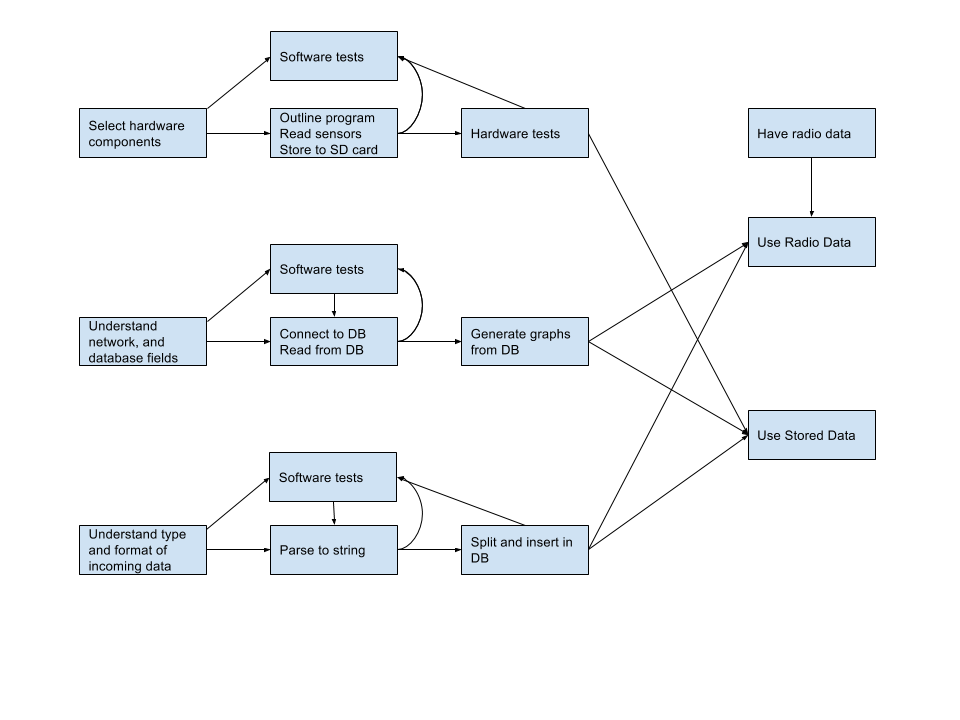
\includegraphics[scale=0.5\textwidth, natwidth=960, natheight=720]{dep_flowchart.png}
\end{figure}


\end{document}
